\documentclass{standalone}
\usepackage{tikz}
\usepackage{float}
\usepackage{amsmath}
\usepackage{lmodern}
\usetikzlibrary{intersections, calc}
\usetikzlibrary{decorations.markings}
\usetikzlibrary{patterns, patterns.meta}
\usetikzlibrary{bbox}

\begin{document}

\centering

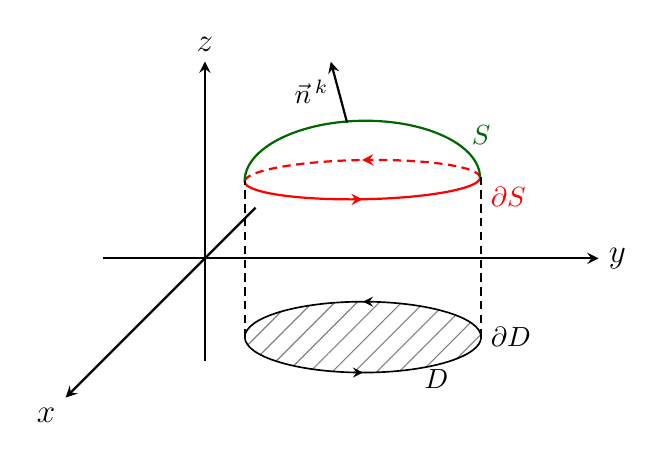
\begin{tikzpicture}
\pgfmathsetmacro{\PtToCm}{0.0352777778}
\tikzset{BigTextFont/.style={font=\large},   % Big text font
    every node/.style={font=\normalsize,text=black},
    arrowstyle/.style={->, >=stealth}}

% custom colors
\definecolor{Green}{rgb}{0.0, 0.4, 0.0}
\definecolor{Red}{rgb}{1, 0, 0}

\pgfmathsetmacro{\OutwardVectorSize}{0.8}       % size of the 3 outward pointed vectors
\pgfmathsetmacro{\DesiredSurfaceWidth}{3}     % desired width of both the upper and lower surface
\pgfmathsetmacro{\ProjectionZ}{-1.0}            % Z-position of the projection
\pgfmathsetmacro{\EpsSafety}{0.10}              % us used to account for thickness lines when getting xmin and xmax values

% ellipse Y to X ratio axis for the bounds
\pgfmathsetmacro{\YXratioUpperSurface}{1/6.0}
% ellipse Y to X relative ratio axis for outer curve of surface
\pgfmathsetmacro{\YXRelativeRatioUpperCurve}{3.0}

% axes
\pgfmathsetmacro{\AxisSize}{5.0} 
\pgfmathsetmacro{\OvershootAxis}{1.3} 
% x and z-axes
\draw[arrowstyle, thick] (-\OvershootAxis,0) -- (\AxisSize,0) node[pos=1, right, BigTextFont] {$y$};
\draw[arrowstyle, thick] (0,-\OvershootAxis) -- (0,\AxisSize * 0.50) node[pos=1, above, BigTextFont] {$z$};
% y-axis (angled)
\pgfmathsetmacro{\ZAxisBeginX}{cos(45) * \OvershootAxis * 0.7}
\pgfmathsetmacro{\ZAxisBeginY}{ sin(45) * \OvershootAxis * 0.7}
\pgfmathsetmacro{\ZAxisEndX}{- cos(45) * 0.5 * \AxisSize}
\pgfmathsetmacro{\ZAxisEndY}{ - sin(45) * 0.5 * \AxisSize}
\draw[arrowstyle, thick] (\ZAxisBeginX, \ZAxisBeginY) -- (\ZAxisEndX, \ZAxisEndY) node[pos=1, below left, BigTextFont] {$x$};

% Upper surface
% save bounding box (as plotbox), this will later be used for checking the max and min of the path. The bezier bounding box is used because it is needed for a proper box when using rotations.
\tikzset{UpperSurfaceTransformation/.style={shift={(2,1)},rotate=1, yscale=1.0 * \YXratioUpperSurface, xscale=1.0}}    % define transformation
\begin{scope}[local bounding box=plotbox, bezier bounding box]
    \path[name path global=myplot, thick,->, UpperSurfaceTransformation] (0,0) circle [radius=0.3];    % create some kind of ellips shape
\end{scope}

% Function: get the min and max x- and y-values of a path 
\def\GetMinAndMaxPath{%

% get the max x- and y-values of a path 
\path[name path=myplotmax] (plotbox.south east) -- (plotbox.north east);    % this is the right bound of the bounding box
\path[name intersections={of=myplot and myplotmax, by={mymax}}];            % get intersection point of right bound bounding box and the shape/path

% extract x- and y- dimension of the intersection point
\newdimen\xmaxPt
\newdimen\ymaxPt 
\pgfextractx{\xmaxPt}{\pgfpointanchor{mymax}{center}}
\pgfextracty{\ymaxPt}{\pgfpointanchor{mymax}{center}}
% convert from Pt to cm
\pgfmathsetmacro{\xmax}{\xmaxPt * \PtToCm}
\pgfmathsetmacro{\ymax}{\ymaxPt * \PtToCm}  

% get the min x- and y-values of a path 
\path[name path=myplotmin] (plotbox.south west) -- (plotbox.north west);    % this is the left bound of the bounding box
\path[name intersections={of=myplot and myplotmin, by={mymin}}];
\newdimen\xminPt 
\newdimen\yminPt 
\pgfextractx{\xminPt}{\pgfpointanchor{mymin}{center}}
\pgfextracty{\yminPt}{\pgfpointanchor{mymin}{center}}  
\pgfmathsetmacro{\xmin}{\xminPt * \PtToCm}
\pgfmathsetmacro{\ymin}{\yminPt * \PtToCm}

% determine scale factor to ensure a certain width
\pgfmathsetmacro{\xwidth}{(\xmax - \xmin)}
\pgfmathsetmacro{\scale}{\DesiredSurfaceWidth / \xwidth}
}

% call function to get proper scaling
\GetMinAndMaxPath{}

% now draw using the proper scaling
\tikzset{UpperSurfaceTransformation/.style={shift={(2,1)},rotate=1, yscale=\scale * \YXratioUpperSurface, xscale=\scale}}
\begin{scope}[local bounding box=plotbox, bezier bounding box]
    \path[name path global=myplot, thick, Green, UpperSurfaceTransformation] (0,0) circle [radius=0.3];
\end{scope}

% draw full part of bounds
\begin{scope}[UpperSurfaceTransformation]
    \clip (- 0.3 - \EpsSafety, -0.3 - \EpsSafety) rectangle (0.3 + \EpsSafety, 0.0);
    \draw[postaction={decorate}, decoration={
    markings,
    mark=at position 0.75 with {\arrow{stealth}},
    }]
    [thick, Red] (0,0) circle [radius=0.3];
\end{scope}
% draw dashed part of bounds
\begin{scope}[UpperSurfaceTransformation]
    \clip (- 0.3 - \EpsSafety, 0.0) rectangle (0.3 + \EpsSafety, 0.3 + \EpsSafety);
    \draw[postaction={decorate}, decoration={
    markings,
    mark=at position 0.25 with {\arrow{stealth}},
    }]
    [thick, Red, densely dashed] (0,0) circle [radius=0.3];
\end{scope}
% draw outer curve
\begin{scope}[shift={(2,1)},rotate=1, yscale=\scale * \YXRelativeRatioUpperCurve * \YXratioUpperSurface, xscale=\scale]
    \clip (- 0.3 - \EpsSafety, 0.0) rectangle (0.3 + \EpsSafety, 0.3 + \EpsSafety);
    \draw[thick, Green] (0,0) circle [radius=0.3];
\end{scope}

% draw 1st outward vector
\pgfmathsetmacro{\StartYVectorA}{\YXRelativeRatioUpperCurve * \YXratioUpperSurface * (\DesiredSurfaceWidth / 2)}    % get the height of the outer curve/ellipse
\draw[postaction={decorate}, decoration={
    markings,
    mark=at position 0.50 with {\node[left] {$\vec{n}^{\,k}$};},
    }]
[thick, arrowstyle, shift={(2,1)},rotate=15] (0, \StartYVectorA) -- (0, \StartYVectorA + \OutwardVectorSize);

% get resulting min and max values for later side wall drawing
\GetMinAndMaxPath{}
\coordinate (UpperLeft) at (\xmin, \ymin);
\coordinate (UpperRight) at (\xmax, \ymax);
\node at (UpperRight) [above, outer sep=0.3cm, text = Green] {$S$};   % parametric equation upper surface
\node at (UpperRight) [below right, text = Red] {$\partial S$};   % parametric equation upper surface

% dashed lines representing projection
\draw[semithick, densely dashed] (\xmin, \ProjectionZ)--(UpperLeft);
\draw[semithick, densely dashed] (\xmax, \ProjectionZ)--(UpperRight);

% projection itself: ellips shape
\pgfmathsetmacro{\ProjectionX}{(\xmax + \xmin) / 2}
\pgfmathsetmacro{\ProjectionRadius}{(\xmax - \xmin) / 2}
\fill[pattern={Lines[angle=45, distance=0.2cm]}, pattern color=gray, shift={(\ProjectionX, \ProjectionZ)}, yscale=0.3] (0, 0) circle[radius=\ProjectionRadius];
\draw[postaction={decorate}, decoration={
    markings,
    mark=at position 0.25 with {\arrow{stealth}},
    mark=at position 0.75 with {\arrow{stealth}},
    }]
[semithick, shift={(\ProjectionX, \ProjectionZ)}, yscale=0.3] (0, 0) circle[radius=\ProjectionRadius];

% nodes projection
\coordinate (LowerRight) at (\xmax, \ProjectionZ);
\node at (LowerRight) [below left, outer sep=0.3cm] {$D$};   % parametric equation upper surface
\node at (LowerRight) [right] {$\partial D$};   % parametric equation upper surface

\end{tikzpicture}

\end{document}